\section{Why Mars}
\frame{\frametitle{Agenda} \tableofcontents[currentsection]}
\subsection{GPGPU}

\begin{frame}
\frametitle{GPU Hardware Trend (1)}
\begin{figure}[ht]
\centering
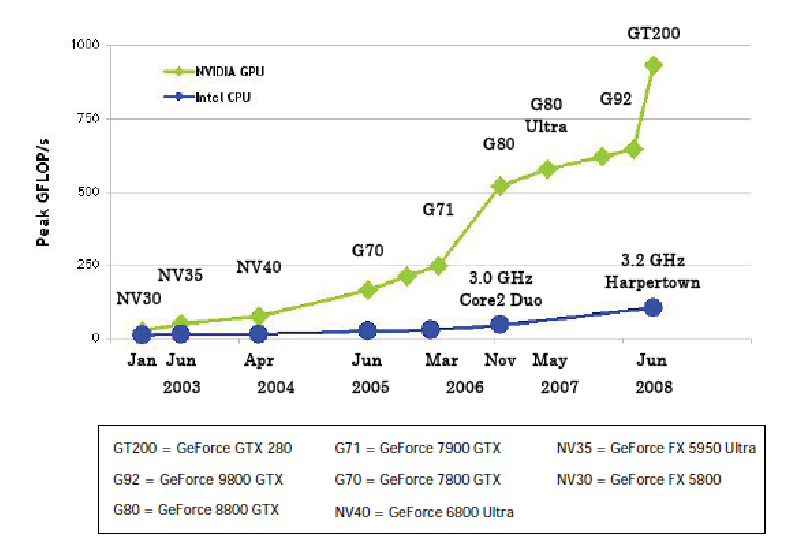
\includegraphics[width=0.70\textwidth]{figure/compute.eps}
\caption{\scriptsize{Floating-Point Operations per Second on NVIDIA GPUs and Intel CPUs.}}
\end{figure}
\vspace{-1em}
\tiny{Source: NVIDA CUDA Programming Guide \cite{CUDA2008}.}
\end{frame}


\begin{frame}
\frametitle{GPU Chip}
\begin{figure}[ht]
\centering
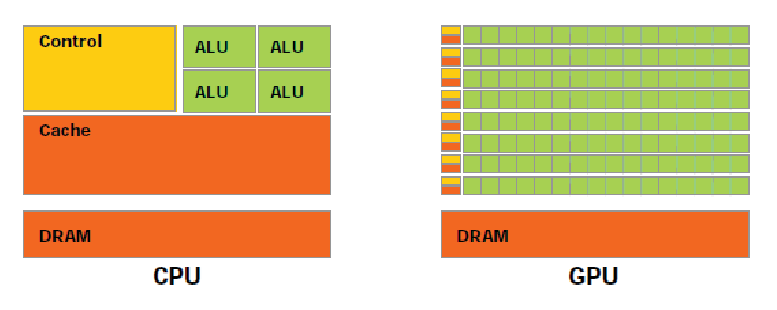
\includegraphics[width=0.90\textwidth]{figure/transistor.eps}
\caption{GPUs devote more transisters to data processing.}
\end{figure}
\tiny{Source: NVIDA CUDA Programming Guide \cite{CUDA2008}.}
\end{frame}

\begin{frame}
\frametitle{GPU Hardware Trend (2)}
\begin{figure}[ht]
\centering
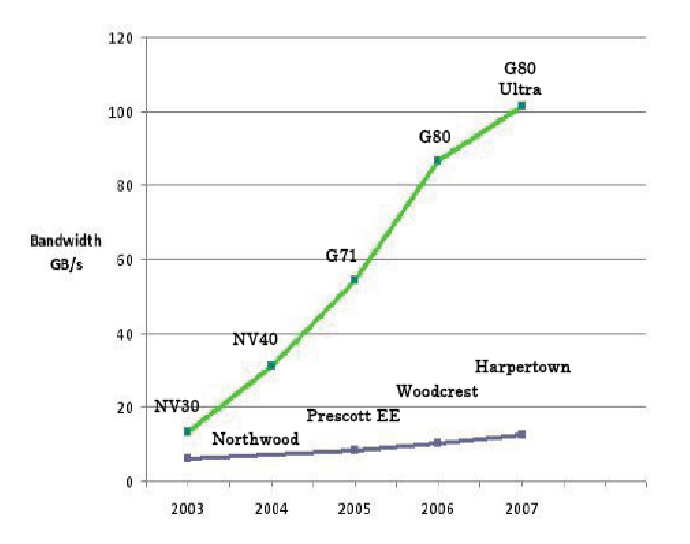
\includegraphics[width=0.60\textwidth]{figure/memory.eps}
\caption{Bandwidth of NVIDIA GPU memory and CPU memory.}
\end{figure}
\tiny{Source: NVIDA CUDA Programming Guide \cite{CUDA2008}.}
\end{frame}


\begin{frame}
\frametitle{General Purpose GPU Computing}
\begin{columns}
\column{0.50\textwidth}
\begin{block}{Many-core Arch for GPUs}
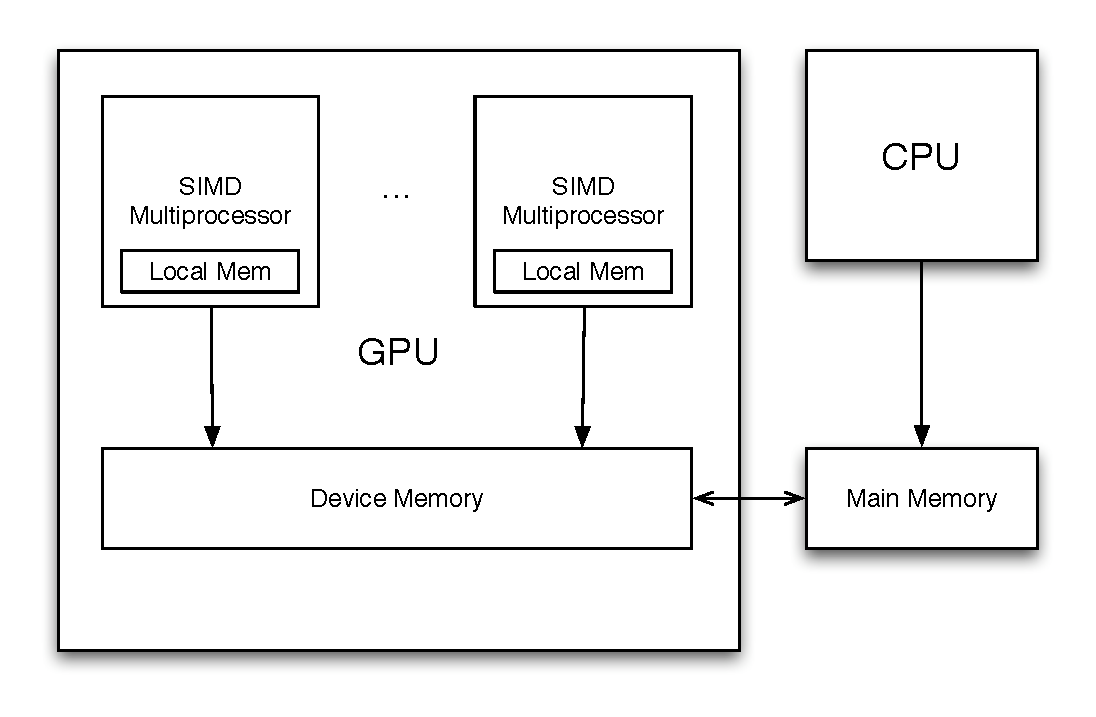
\includegraphics[width=1.0\textwidth]{figure/gpuarch.eps}
\end{block}
\column{0.50\textwidth}
\begin{block}{Programability}<2>
\begin{itemize}
\item NVIDIA CUDA
\item AMD Brook+
\item OpenCL
\item More... 
\end{itemize}
\end{block}
\end{columns}
\end{frame}

\begin{frame}
\frametitle{Non-Graphics Workloads on GPUs}
Owens et al. \cite{Owens2007} \textbf{A Survey of General-Purpose Computation on Graphics Hardware}
\begin{itemize}
\item Linear algebra
\item Finance
\item Database query
\item Machine Learning
\item More...
\item \alert{Data Parallel} programs on SIMD multiprocessors.
\end{itemize}
\end{frame}

\subsection{MapReduce}
\begin{frame}
\frametitle{Map Function and Reduce Function}
Jeffrey Dean and Sanjay Ghemawat, \textbf{MapReduce: Simplified Data Processing on Large Clusters. OSDI'04}. \cite{Dean2008}
\begin{quote}
{\bf Map}(void *{\em doc}) \{ \\
1: {\bf for} each word {\em w} in {\em doc} \\
2: \hspace{3mm} {\bf EmitIntermediate}({\em w}, {\em 1}); // count each word once \\
\} \\
{\bf Reduce}(void *{\em word}, Iterator {\em values}) \{ \\
1: int {\em result} = 0; \\
2: {\bf for} each {\em v} in {\em values} \\
3: \hspace{3mm} {\em result} += {\em v}; \\
4: {\bf Emit}({\em word}, {\em result}); // output {\em word} and its count \\
\}
\end{quote}
\end{frame}

\begin{frame}
\frametitle{MapReduce Workflow}
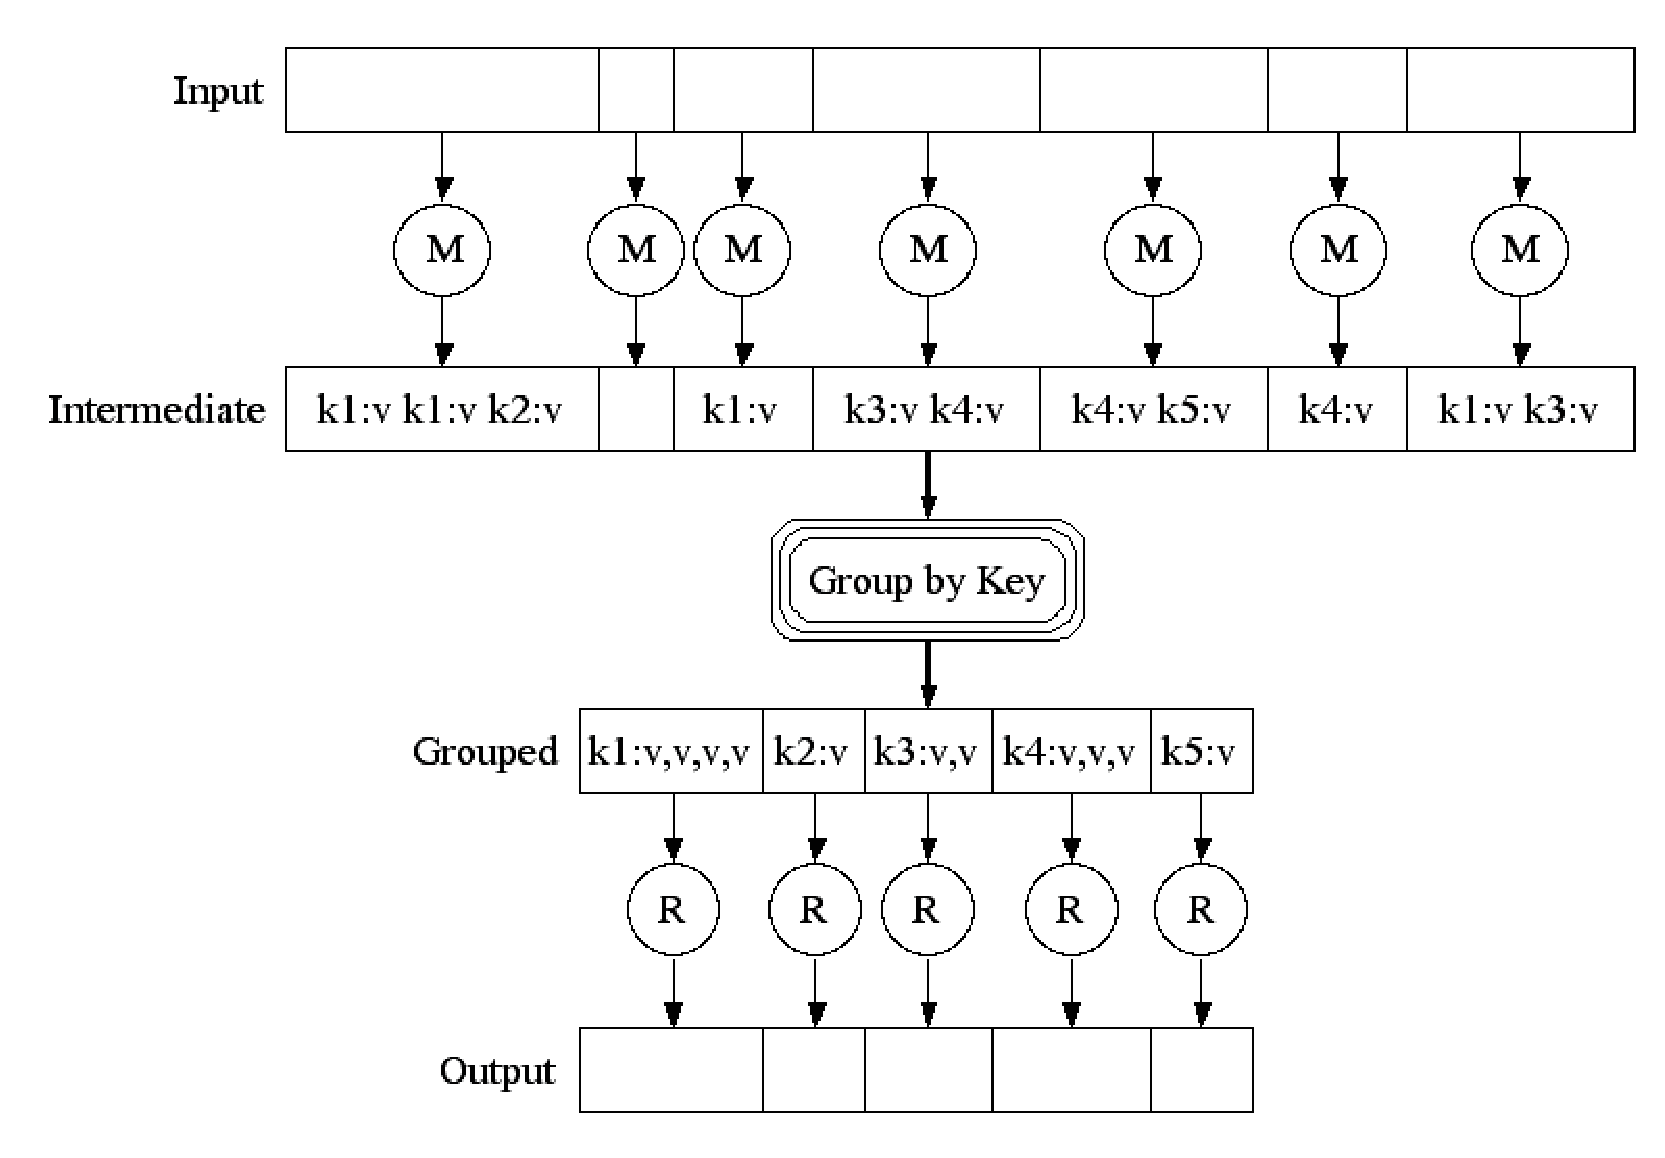
\includegraphics[width=0.80\textwidth]{figure/mr_workflow.eps}
\\\tiny{{\em Source - http://labs.google.com/papers/mapreduce-osdi04-slides/index-auto-0007.html}}
\end{frame} 

\begin{frame}
\frametitle{Implementations of MapReduce}
\begin{itemize}
\item<1-> Distributed Environment
\begin{itemize}
\item Google MapReduce
\item Apache Hadoop (Yahoo\!, Facebook, ...)
\item MySpace Qizmt
\end{itemize}
\item<2-> Multi\-core CPU
\begin{itemize}
\item Phoenix from Stanford, HPCA'07 \cite{Ranger2007}/IISWC'09 \cite{Yoo2009}.
\end{itemize}
\item<3-> Cell BE
\item<3-> FPGA
\item<4-> GPUs
\begin{itemize}
\item From UC-Berkeley, STMCS'08 \cite{Kruijf2007}
\item Merge, from Intel, ASPLOS'08 \cite{Linderman2008}
\end{itemize}
\end{itemize}
\end{frame}
